\documentclass[xcolor=table,aspectratio=169,dvipsnames,english]{beamer}
\usepackage{bm}
\usepackage[utf8]{inputenc}
\usepackage{color}

% Biblatex, sucks, but it's apparently the only way to get DOI/URLs displayed with beamer and only moderately fuck up the formatting:
% https://tex.stackexchange.com/a/552458/27977
\usepackage[sorting=none,style=numeric,doi=true]{biblatex}
\addbibresource{bib.bib}
\renewcommand*{\bibfont}{\footnotesize}

\usepackage{makecell}
\usepackage{siunitx}
\usepackage{todonotes}

\sisetup{per-mode=symbol, detect-all, range-units = single} % will use the current font for typesetting
\newcommand\SIci[5]{\SI{#1}{#2}, {#3}CI: \SIrange{#4}{#5}{#2}}

\DeclareSIUnit[number-unit-product = {}]
	\vg{vg}


% Single-session PythonTeX codeblocks
\newcounter{pysessioncounter}
\newcommand{\sessionpy}{%
	  \edef\sessionpysession{session\arabic{pysessioncounter}}%
	    \stepcounter{pysessioncounter}%
	      \expandafter\py\expandafter[\sessionpysession]}


% Article-specific configuration
\begin{pythontexcustomcode}[begin]{py}
DOC_STYLE="slides/main.conf"
pytex.add_dependencies(
	DOC_STYLE,
	'slides/2x1.conf',
	'slides/2x1_coordinates.conf',
	)
\end{pythontexcustomcode}

% Custom beamer styling and colors
\setbeamersize{text margin left=0.8em,text margin right=0.8em}
\setbeamertemplate{bibliography item}{\insertbiblabel}

\usecolortheme[RGB={199,199,199}]{structure}
\usetheme{Dresden}

\captionsetup[figure]{labelformat=empty}

\definecolor{dy}{RGB}{202,202,0}
\definecolor{rsblue}{HTML}{00a3cc}
\definecolor{mg}{gray}{0.30}
\definecolor{lg}{gray}{0.60}
\definecolor{vlg}{gray}{0.78}
\definecolor{tlg}{gray}{0.88}

\setbeamercolor{caption name}{fg=lg}
\setbeamercolor{caption}{fg=lg}
\setbeamercolor{author}{fg=lg}
\setbeamercolor{institute}{fg=lg}
\setbeamercolor{date}{fg=lg}
\setbeamercolor{title}{fg=mg}
\setbeamertemplate{caption}{\centering\insertcaption\par}
\setbeamertemplate{navigation symbols}{}

% Navigation symbols are too far down by default
% To further adjust edit the pt numbers before and after `\insertnavigation`
\makeatletter
\defbeamertemplate*{headline}{my miniframes theme}
{%
        \begin{beamercolorbox}[colsep=1.5pt]{upper separation line head}
        \end{beamercolorbox}
        \begin{beamercolorbox}{section in head/foot}
                \vskip1pt\insertnavigation{\paperwidth}\vskip3pt
        \end{beamercolorbox}%
        \ifbeamer@theme@subsection%
                \begin{beamercolorbox}[colsep=1.5pt]{middle separation line head}
                \end{beamercolorbox}
                \begin{beamercolorbox}[ht=2.5ex,dp=1.125ex,%
                        leftskip=.3cm,rightskip=.3cm plus1fil]{subsection in head/foot}
                        \usebeamerfont{subsection in head/foot}\insertsubsectionhead
                \end{beamercolorbox}%
        \fi%
        \begin{beamercolorbox}[colsep=1.5pt]{lower separation line head}
        \end{beamercolorbox}
}
\makeatother


\title[Whole-Brain Map and Assay Parameter Analysisof Mouse VTA Dopaminergic Activation --- ISMRM 2020]{A Whole-Brain Map and Assay Parameter Analysisof Mouse VTA Dopaminergic Activation}
\subtitle{ISMRM 2020\\\href{https://bitbucket.org/TheChymera/opfvta}{\small\texttt{[ bitbucket.org/TheChymera/opfvta ]}}}
\author[Horea-Ioan Ioanăș]{Horea-Ioan Ioanăș\\\href{https://twitter.com/TheChymera}{\small\texttt{[ @TheChymera ]}}}
\institute{Institute for Biomedical Engineering, ETH and University of Zurich}
\date{}
\begin{document}
	\begin{frame}
		\titlepage
	\end{frame}
	\section{Background}
		\subsection{The dopaminergic (DA) system — a critical node for controlling brain function}
			\begin{frame}{Key Features of the DA System}
				\begin{figure}
					\begin{subfigure}{.46\textwidth}
						\vspace{-.5em}
						\centering
						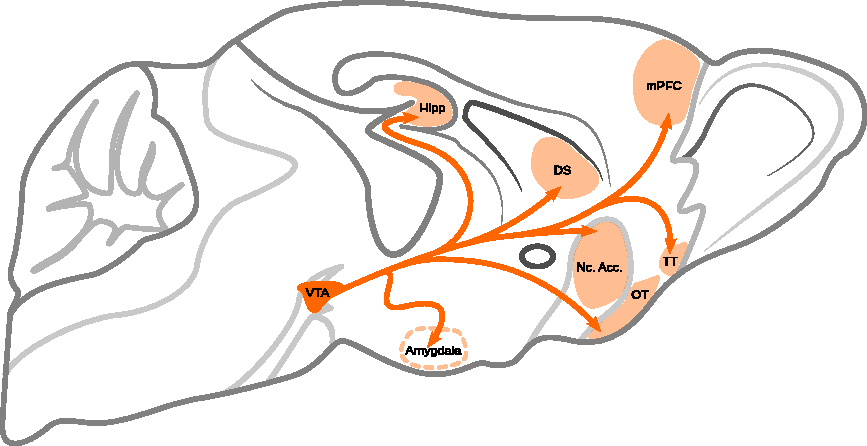
\includegraphics[width=\textwidth]{img/model_literature}
						\vspace{-2em}
						\caption{VTA DA projections}
					\end{subfigure}
					\begin{subfigure}{.53\textwidth}
						\vspace{-2.75em}
						\centering
						\includedot[width=\textwidth]{data/network_model}
						\vspace{-2.5em}
						\caption{Weighted graph model}
					\end{subfigure}
					\vspace{-.75em}
				\end{figure}
				\begin{itemize}
					\item Key to the etiology of addiction \cite{DiChiara1999}, attentional control \cite{Nieoullon2002}, and motivation \cite{Salamone1994}.
					\item Evolutionarily well-conserved \cite{Yamamoto2011}.
					\item Small number of functionally similar and widely projecting cells ($\approx4,000$ in mice).
				\end{itemize}
			\end{frame}
			\begin{frame}{Objectives}
				\begin{minipage}{.38\textwidth}
					\vspace{-3em}
					\centerline{I.}
					Establish a \underline{reusable assay} and workflow implementation for VTA DA functional imaging in mice.

					\vspace{2.5em}
					\centerline{II.}
					Publish a \underline{reference neurophenotype} for VTA DA neurotransmission.
				\end{minipage}\hfill
				\begin{minipage}{.6\textwidth}
					\vspace{-1.5em}
                                        \begin{figure}[htp] \centering{
                                                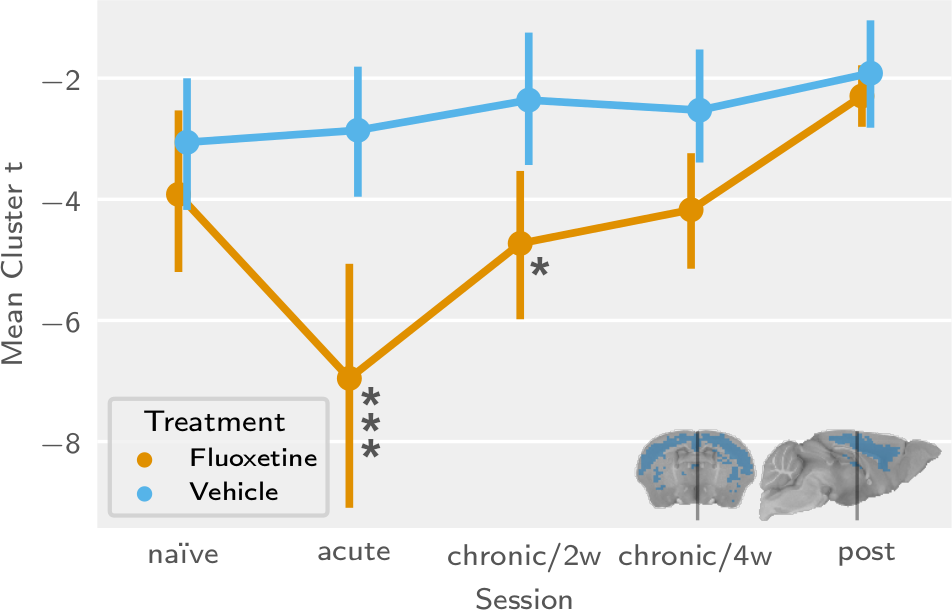
\includegraphics[width=\textwidth]{img/cortical_t.png}}
						\vspace{-1.5em}
						\caption{\centering Serotonergic neurophenotype used for psychopharmacological profiling (ISMRM 2018) \cite{phd}}
                                        \end{figure}
                                \end{minipage}
			\end{frame}
	\section{Methods}
		\subsection{Proof of principle for mouse VTA DA opto-fMRI}
			\begin{frame}{}
				\begin{figure}
					\vspace{.7em}
					\centering
					\includegraphics[width=\textwidth]{img/optogenetics}
					\caption{Workflow for MR-compatible optogenetic targeting using DAT-Cre mice \cite{dat}}
				\end{figure}
			\end{frame}
	\section{Results}
		\subsection{A functional dopaminergic neurophenotype in the mouse}
			\begin{frame}{}
				\sessionpy{pytex_subfigs(
					[
						{'script':'scripts/taskgroup.py', 'conf':'slides/2x1.conf', 'options_pre':'{.48\\textwidth}',
							'options_pre_caption':'\\vspace{-2.1em}',
							'caption':'Task group comparison for animals targeted at all explored combinations of implant coordinates.',
							},
						{'script':'scripts/implant_coordinates_block.py', 'conf':'slides/2x1_coordinates.conf', 'options_pre':'{.48\\textwidth}',
							'options_pre_caption':'\\vspace{-1.1em}',
							'caption':'Block stimulation trial coordinates (inner dots indicate best category group).',
							},
						],
					environment='figure',
					)}
			\end{frame}
			\begin{frame}{Block Stimulation of Best Implant Group — as per VTA Activation}
				\vspace{-.3em}
				\sessionpy{pytex_subfigs(
					[
						{'script':'scripts//map_block_filtered_controlled.py', 'conf':'slides/2x1_map.conf', 'options_pre':'{.48\\textwidth}',
							'options_pre_caption':'\\vspace{-2.5em}',
							'caption':'Centered on VTA.',
							},
						{'script':'scripts/map_block_filtered_controlled_auto.py', 'conf':'slides/2x1_map.conf', 'options_pre':'{.48\\textwidth}',
							'options_pre_caption':'\\vspace{-2.5em}',
							'caption':'Centered on largest cluster.',
							},
						],
					environment='figure',
					)}
			\end{frame}
			\begin{frame}{Seed-Based Functional Connectivity Analysis}
				\vspace{-.6em}
				\sessionpy{pytex_subfigs(
					[
						{'script':'scripts//map_block_filtered_seed.py', 'conf':'slides/2asymmetric_map.conf', 'options_pre':'{.4\\textwidth}',
							'options_pre_caption':'\\vspace{-1.3em}',
							'caption':'Centered on VTA, seed region in green.',
							},
						{'script':'scripts/distributions_block_filtered_seed.py', 'conf':'slides/2asymmetric_distributions.conf', 'options_pre':'{.59\\textwidth}',
							'options_pre_caption':'\\vspace{-2.5em}',
							'caption':'Centered on largest cluster.',
							},
						],
					environment='figure',
					)}
			\end{frame}
			\begin{frame}{}
				\vspace{-.45em}
				\sessionpy{pytex_fig(
					'scripts/features_filtered_coronal.py',
					conf='slides/coronal.conf',
					options_pre_caption='\\vspace{-1.3em}',
					caption='
						\\scriptsize
						VTA functional/structural projection contrast.
						Parcellation correlation of population averages: $\\rho\\!=\\!0.52, p\\!=\\!1\\!\\times\\!10^{22}$
						',
					label='ffcc',
					options_pre='\\centering\n',
					environment='figure',
					figure_format='pdf',
					)}
			\end{frame}
	\section{Conclusions}
		\subsection{A functional dopaminergic neurophenotype in the mouse}
			\begin{frame}{Key Contributions to Preclinical DA Modelling}
				\begin{itemize}
					\item Proof of principle for VTA DA opto-fMRI in mice.
					\item Determined optimal sensitivity parameters for the assay.
					\item Produced reference neurophenotype in standard space.
					\item Documented overall coherence with, yet key deviations (esp. dorsomedial striatum) from structural projection map — potentially on account of partial SNc activation.
					\item Seed-based functional connectivity analysis facilitates accurate disambiguation of VTA activity, but suffers from SNR loss in projection areas.
				\end{itemize}
			\end{frame}
%	\section{Features}
%		\subsection{Create All Graphic Elements Directly from Source.}
%			\begin{frame}{}
%				\py{pytex_fig('scripts/3dplot.py', conf='slides/3dplot.conf', label='3dplot', caption='A 3D plot.')}
%			\end{frame}
%			\begin{frame}{}
%				\vspace{-.3em}
%				\setlength\abovecaptionskip{-5pt}
%				\py{pytex_fig('scripts/bsc_percentage.py', conf='slides/tall.conf', label='bsc_percentage', caption='Percentage of Bachelor’s degrees conferred to women in the U.S.A. by major (1970-2011).')}
%			\end{frame}
%			\begin{frame}{And So Much More}
%				\py{pytex_subfigs(
%					[
%						{'script':'scripts/vc_violin.py', 'label':'vcv', 'conf':'slides/1col.conf', 'options_pre':'{.48\\textwidth}',
%						},
%						{'script':'scripts/vcc_violin.py', 'label':'vccv','conf':'slides/1col.conf', 'options_pre':'{.48\\textwidth}',
%						},
%						],
%					environment='figure',
%					label='fig:vc',
%					)}
%			\end{frame}
	%\section{References}
		% We use biblatex here, see `slides/header.tex`
		%\bibliographystyle{unsrt}
		%\bibliography{./bib}
		\tiny
		\printbibliography
\end{document}
